\chapter{Formulação do Problema}\label{chapter:formulacaoDoProblema}

O desenvolvimento da plataforma \textit{Corporate Collaboration} pretende atingir certos requisitos, de forma a poder enquadrá-la no mercado 
atual. 


\section{Estado da Arte}\label{sec:estadoDaArte}
As plataformas de colaboração existentes no mercado atual tais como a \textit{Microsoft SharePoint} ou a \textit{BaseCamp} apresentam um elevado nível de complexidade, 
incluindo ferramentas como calendários partilhados, partilha de ficheiros, mensagens instantâneas, armazenamento na \textit{cloud}, video-conferência, entre outros. 

\par
A aplicação desenvolvida neste âmbito não procura igualar todas as funcionalidades das plataformas já existentes, 
mas sim, agilizar a dinâmica de atividades internas que ocorrem diariamente nas empresas. 
Visa, essencialmente, facilitar a procura de pessoas para cumprir certas necessidades que existam no âmbito das atividades internas da empresa, 
necessidades estas que permitem definir uma tarefa que tem de ser realizada ou um evento que será organizado no contexto da dinâmica interna da empresa. 

\par 
Estas necessidades são auxiliadas por recursos que permitem gerir candidaturas e participantes das mesmas, 
assim como apresentar informações sobre alojamento, refeições, transporte e localização, se for caso disso.

\newpage

\section{Análise de Requisitos}\label{sec:requisitos}

As funcionalidades principais da plataforma \textit{Corporate Collaboration} estão representadas na figura~\ref{fig:uc:generalActions}

\begin{figure}[H]
    \centering
    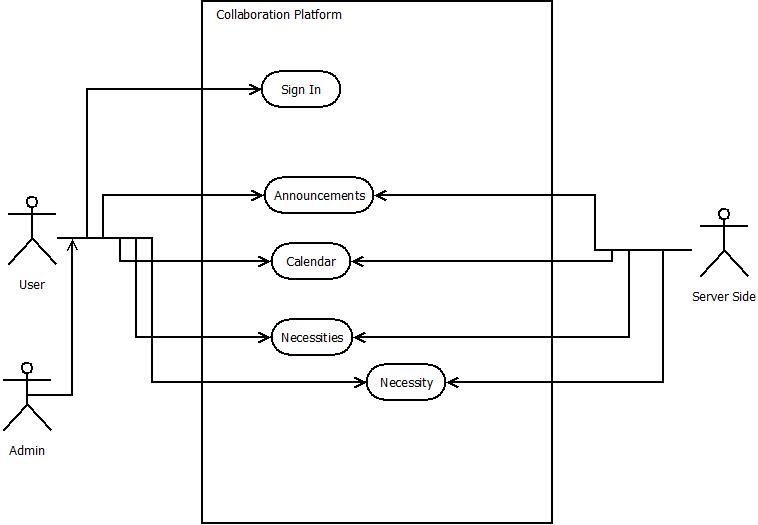
\includegraphics[scale=0.6]{figures/General Actions.jpeg}
    \caption{\textit{Use Case} --- Ações gerais.}\label{fig:uc:generalActions}
\end{figure}

\newpage

\subsection{Módulos constituintes da \textit{Collaboration Platform} e \textit{roles} associados}

A plataforma de colaboração desenvolvida é constituída por dois módulos denominados \textit{back-office} e \textit{UserEndPoints}. 

\par
O acesso ao \textit{back-office} é realizado apenas por utilizadores com permissões de administrador ou de \textit{owner}. 
Um \textit{owner} é descrito como a entidade superior da hierarquia de \textit{roles}, só existe um utilizador com esta permissão. 
Um administrador é um utlizador com permissões superiores a um utilizador comum, permissões estas descritas na figura~\ref{fig:uc:user_admin_scheme}. 

\par
No módulo \textit{back-office} são realizadas todas as operações de manutenção e funcionamento da plataformma colaborativa.

\par
O módulo \textit{UserEndPoints} suporta o acesso ás principais funcionalidades que a \textit{Collaboration Platform} apresenta e pode ser acedido por todos os utilizadores registados na aplicação.

\par
As funcionalidades a que cada \textit{role} (utilizador comum, administrador e \textit{owner}) tem acesso são descritas na figura~\ref{fig:uc:user_admin_scheme}.

\begin{figure}[H]
    \centering
    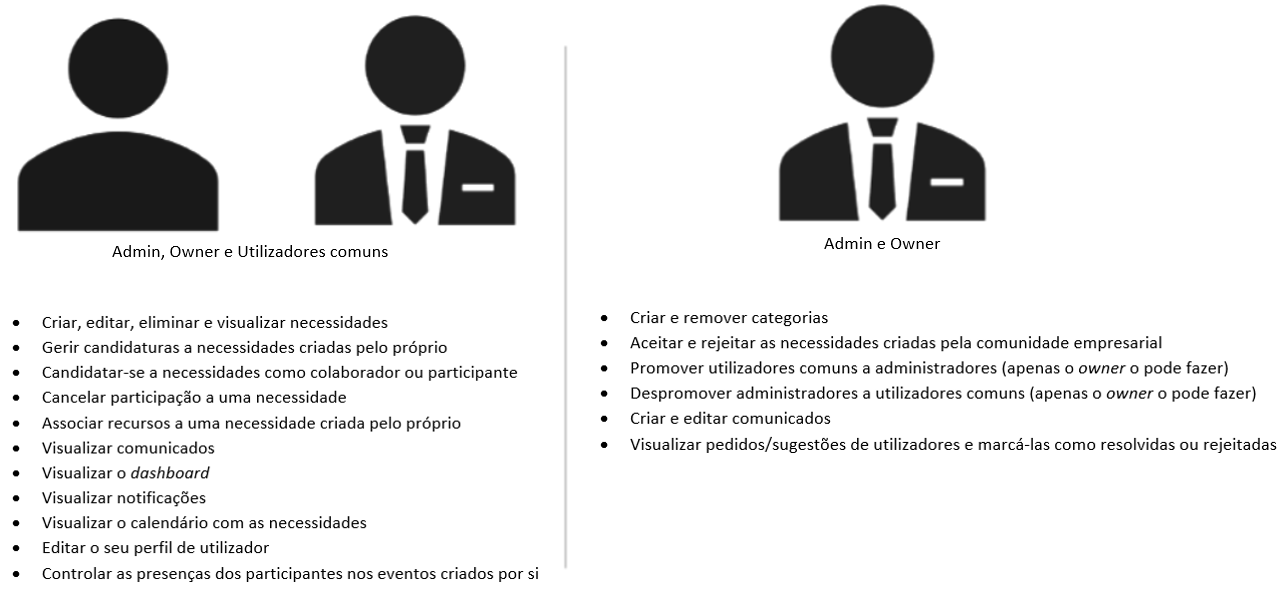
\includegraphics[scale=0.4]{figures/user_admin_owner_scheme.png}
    \caption{Funcionalidades a que cada \textit{Role} tem acesso.}\label{fig:uc:user_admin_scheme}
\end{figure}

\newpage

\subsection{Registo e Autenticação}\label{subsec:login}

Para desenvolver a funcionalidade de registo e autenticação na plataforma de colaboração é necessário existir uma tabela 
na base de dados que guarde as credenciais e informação básica de cada utilizador, nomeadamente 
o \textit{email}, \textit{password}, \textit{username}, primeiro e último nome. 
Esta tabela tanto serve para efeitos de registo de um utilizador, como para verificação posterior da sua autenticação. 
Os utilizadores não necessitam de fazer registo na aplicação, visto que nesta plataforma é suposto utilizarem 
as mesmas credenciais atribuidas pela empresa, para e-mail e autenticação nas outras aplicações internas.

Relativamente ao ecrã de \textit{Login} ilustrado na figura~\ref{fig:uc:login}, este suporta:

\begin{itemize}
    \item Duas caixas de texto onde o utilizador introduz o seu e-mail e password.
    \item Um botão identificado como \textit{Login} que desencadeia o processo de verificação das credencias introduzidas.
\end{itemize}

\begin{figure}[H]
    \centering
    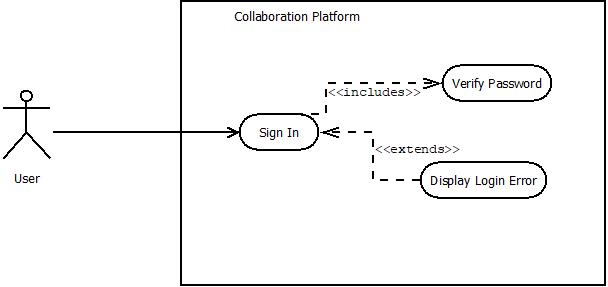
\includegraphics[scale=0.6]{figures/Login Use Case.jpeg}
    \caption{\textit{Use Case} --- \textit{Login}.}\label{fig:uc:login}
\end{figure}

\newpage

\subsection{Manutenção da aplicação e \textit{Back-Office}}\label{subsec:manutencao_e_back-office}

Com o objetivo de realizar operações de manutenção e operações que requerem privilégio superior ao de um utilizador comum foi implementado um novo módulo, denominado \textit{back-office}. 

\par 
Um utilizador com permissões de administrador ou de \textit{owner} tem acesso ao \textit{back-office} onde pode criar ou remover categorias, analisar as necessidades criadas pela comunidade empresarial e escolher se as mesmas são aceites e divulgadas na plataforma ou eliminadas,
ver todos os utilizadores da plataforma colaborativa e as suas permissões (sendo que o \textit{owner} pode alterá-las) e analisar mensagens produzidas por um dado utilizador comum com pedidos/sugestões para os utilizadores com permissões superiores (\textit{admin ou owner}).  

\begin{figure}[H]
    \centering
    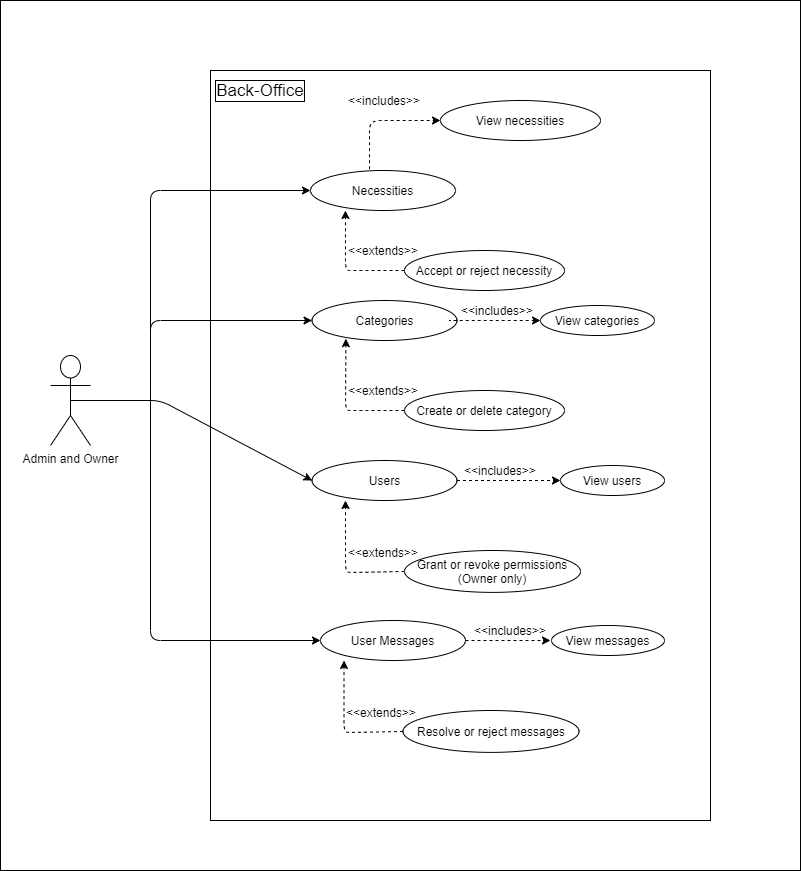
\includegraphics[scale=0.5]{figures/back-office_use_case (1).png}
    \caption{\textit{Use Case} --- Back-Office.}\label{fig:uc:backoffice_use_case}
\end{figure}

\newpage

\subsection{\textit{Home Page --- Dashboard}}\label{subsec:dashboard}

No contexto do módulo \textit{UserEndPoints}, é no domínio do mesmo que se concentram as principais funcionalidades da \textit{Collaboration Platform}, descritas doravante. 
Estas são acessíveis a todos os utilizadores autenticados e, logo após o \textit{login}, o utilizador será redirecionado para um novo ecrã que irá conter um \textit{dashboard} com o intuito de organizar e 
apresentar a informação de uma forma apelativa. 
\par
Este ecrã apresenta o número total de utilizadores registados na aplicação e o total de necessidades criadas até ao momento organizadas por nível de prioridade (Low, Medium e High). 
Ao carregar num destes níveis de prioridade especificados no ecrã o utilizador é redirecionado para o ecrã das necessidades, apresentando a lista das mesmas com o filtro correspondente à prioridade selecionada. 
\par
Este \textit{Dashboard} contém ainda um gráfico circular que demonstra uma estatística relativa ao número de necessidades que existem em cada categoria. A seleção de uma das categorias deste gráfico redirecionará o utilizador para o ecrã das necessidades, apresentando a lista das mesmas com o filtro correspondente à categoria selecionada.
\par
É também apresentado o \textit{top 5} de necessidades criadas mais recentemente e aceites por utilizadores com permissões de administrador (ou pelo \textit{owner}), onde cada uma tem um link que redireciona o utilizador para o detalhe da mesma. 
\par
Por fim, é apresentado o top 5 de utilizadores que têm mais necessidades criadas para cada um dos níveis de prioridade que uma necessidade pode ter.

\newpage

\subsection{Registo das necessidades internas da empresa, gestão de candidaturas, associação de recursos, notificações e integração com o google maps}\label{subsec:necessitiesCandidatesNotificationsGoogleMaps}

A principal funcionalidade que a \textit{Collaboration Platform} apresenta é a de gestão das necessidades internas de uma empresa, descrita na figura~\ref{fig:uc:necessities}.

\par
O conceito subjacente a esta funcionalidade é o de necessidade (\textit{necessity}), que permite virtualizar uma necessidade interna, assegurando os seus detalhes e características.
Um utilizador autenticado tem a possibilidade de ver necessidades criadas pela comunidade e criar, editar, eliminar ou arquivar uma necessidade da sua autoria.

\begin{figure}[H]
    \centering
    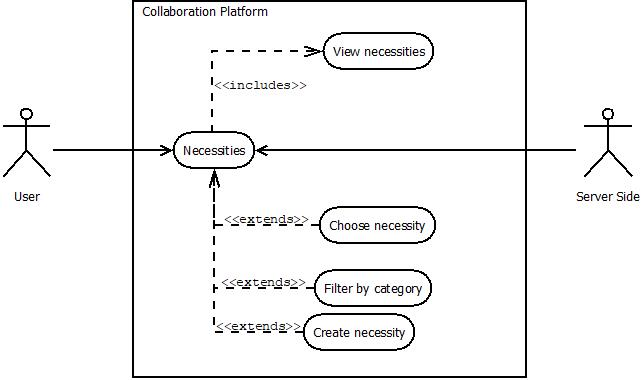
\includegraphics[scale=0.6]{figures/Necessities.jpeg}
    \caption{\textit{Use Case} --- Necessidades.}\label{fig:uc:necessities}
\end{figure}

\par
Posto isto, é fundamental que exista um ecrã que apresente todas as necessidades criadas pela comunidade da empresa. 
Um utilizador, caso queira registar uma necessidade, irá escolher a categoria que melhor se adequa à mesma. 


\begin{figure}[H]
    \centering
    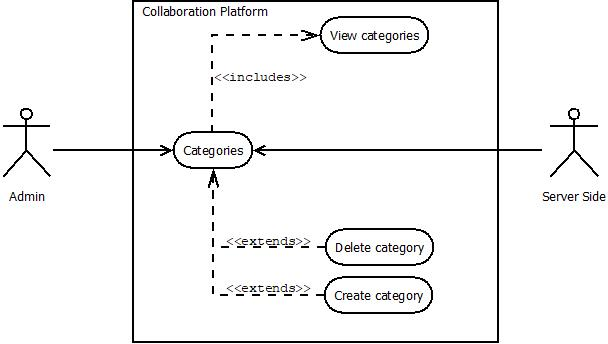
\includegraphics[scale=0.6]{figures/Categories use case.jpeg}
    \caption{\textit{Use Case} --- Categorias.}\label{fig:uc:categories}
\end{figure}

Deste modo, definimos um conjunto de filtros que podem ser conjugados de modo a permitir um melhor agrupamento e organização das necessidades. 
O primeiro consiste na filtragem por categorias, como por exemplo \textit{Brown Bags}, 
\textit{Qualification Offers}, \textit{Software Components Development} ou \textit{Planning of Events}. 
Apenas um utlizador com permissões de administrador ou o \textit{owner} podem criar ou eliminar novas categorias no \textit{back-office} da aplicação, como descrito na figura~\ref{fig:uc:categories}.
\par
Foi ainda definido um segundo filtro que poderá tomar os valores \textit{High}, \textit{Medium} ou \textit{Low}, 
correspondentes ao grau de prioridade com que as necessidades foram criadas. 
\par
A seleção dos filtros irá levar a uma atualização da lista para conter apenas necessidades que se enquadrem nessa mesma seleção. 
\par
Este ecrã apresenta ainda um botão que servirá para criar uma nova necessidade, criação esta acessível a todos os utilizadores autenticados, 
que decorrerá num novo ecrã e que terá como opção (obrigatória) de criação os filtros a qual associar a nova necessidade. 
\par
Em cada necessidade existe a possibilidade de associar recursos com informações sobre alojamento, refeições, localização do evento ou transporte para o local onde a mesma se irá realizar. Todos os recursos, com exceção do recurso transporte, têm associado um mapa do \textit{Google Maps} onde os utilizadores podem fornecer informações sobre localização.
\par
Ao clicar numa necessidade, será apresentado um novo ecrã com os detalhes da mesma, com os recursos associados e também a possibilidade do utilizador se candidatar como colaborador ou participante da necessidade, dependendo da fase em que a mesma se encontra. O autor da necessidade irá receber a notificação de que existe um novo candidato, 
dando-lhe a opção de após carregar na notificação ser redirecionado para o ecrã de detalhe da necessidade onde pode observar os candidatos. 

\par
Ao criar uma necessidade o autor tem a possibilidade de escolher se todas as candidaturas à necessidade em causa são aceites automaticamente ou se o próprio escolhe os candidatos com base na descrição dada pelos mesmos.  
O candidato irá receber uma notificação nos casos em que a necessidade for fechada/cancelada, e quando a sua candidatura for aceite/recusada. 
Terá também a possibilidade de ver quem já se candidatou á necessidade criada pelo próprio no ecrã de detalhe na \textit{aba} dos participantes, estando candidatos a colaboradores separados de candidatos a participantes. 
\par
O ecrã que permite mostrar as notificações associadas a cada utilizador é acedido ao carregar no ícone em forma de sino presente na barra da aplicação. Este ícone tem um pequeno contador associado que indica o número de notificações pendentes que cada utilizador tem e, quando pressionado, é apresentado o ecrã das notificações onde as mesmas são apresentadas na forma de uma lista. 

\begin{figure}[H]
    \centering
    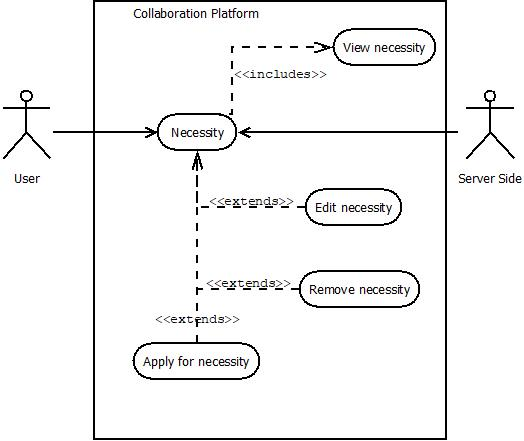
\includegraphics[scale=0.6]{figures/Necessity.jpeg}
    \caption{\textit{Use Case} --- Necessidade.}\label{fig:uc:necessity}
\end{figure}

Exemplificando, para criar uma necessidade cuja motivação é um eventos ou uma feira de emprego, o utilizador seleciona a categoria \textit{Planning of events}.

Se por outro lado, tiver  o objetivo de realizar apresentações informais de partilha de conhecimento, o utilizador seleciona a categoria \textit{Brown Bags}. 
\par
Todos os utilizadores devidamente autenticados podem candidatar-se ás necessidades existentes, tendo livre acesso para leitura dos detalhes de cada uma. 
\par
O autor de uma necessidade é o utilizador que a criou. Tem as permissões de poder editar, eliminar ou arquivar a mesma, associar recursos e gerir participantes/colaboradores.
\par
No contexto da necessidade, é definida uma linha temporal que consiste numa primeira fase de candidaturas para escolha do orientador 
(ou orientadores), dando origem ao conceito de \textit{"Collaborator"}.  
Um utilizador adquire este cargo, para uma dada necessidade, após ver a sua candidatura aceite pelo autor da mesma. Este utilizador adquire as mesmas permissões de um participante comum e adquire também as permissões de poder editar a necessidade, com exceção da data do evento e de aceitar ou rejeitar participantes. 
\par
O autor de uma necessidade, no ecrã de detalhe da mesma, terá acesso a quem se candidatou para a orientar (ser \textit{Collaborator} nesta necessidade), podendo escolher um ou mais orientadores 
com base na descrição apresentada pelos mesmos. 
A linha temporal definida no contexto de uma necessidade tem ainda uma segunda fase de candidaturas para permitir o acesso como participante. 
Um utilizador torna-se um participante após ser aceite pelo autor no caso de haver filtragem dos candidatos ou, no caso de não se verificar a opção de haver filtragem, a candidatura é aceite automaticamente. 
O cargo de participante permite também a participação nos recursos associados à necessidade.
\par
Todos os utilizadores autenticados podem ver quem foi aceite como participante e como colaborador.
\par
Com o intuito de poder realizar a marcação de presenças de cada um dos participantes a uma necessidade, foi introduzido na plataforma o conceito de \textit{QR Code}. 
Os mesmos são gerados individualmente para cada participante no dia em que o evento terá lugar e os utilizadores com papéis de autor ou colaborador da necessidade podem fazer scan dos \textit{QR Codes} de cada um dos participantes.
Após o scan de um \textit{QR Code} de um dado participante, o mesmo será sinalizado como presente.

\newpage

\subsection{Divulgação e calendarização das necessidades}

Com o objetivo de divulgar e calendarizar as necessidades internas da empresa, a barra de navegação da aplicação apresenta um botão com o nome \textit{Calendar} que, quando pressionado, 
redireciona o utilizador para um ecrã que apresenta um calendário com o qual ele poderá interagir. 
\par
Neste calendário são apresentados todos os eventos organizados, na sua respetiva data, e existe a possibilidade de filtrar os eventos em que o utilizador participará. 
\par
Após a seleção de um dia no calendário, são apresentadas as necessidades, dando a possibilidade ao utilizador de ver os detalhes individuais após carregar numa delas, 
num novo ecrã.
As ações possíveis de utilização deste calendário estão presentes na figura~\ref{fig:uc:calendar}. 
Uma necessidade, no contexto do calendário, é referida como um evento numa determinada data. 

\begin{figure}[H]
    \centering
    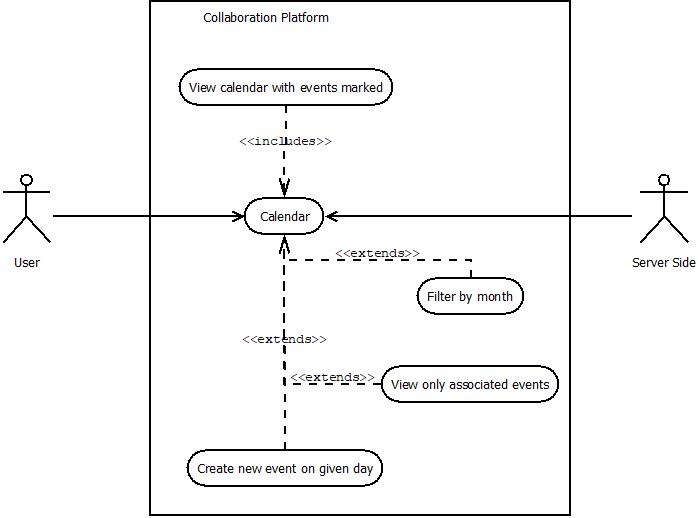
\includegraphics[scale=0.6]{figures/Calendar use case.jpeg}
    \caption{\textit{Use case} --- Calendário.}\label{fig:uc:calendar}
\end{figure}

Para ser possível divulgar as necessidades da empresa de forma uniforme por todos os seus colaboradores, a barra de navegação da aplicação apresenta
um botão denominado \textit{Announcements} que, quando pressionado, abre um ecrã que contém os comunicados sobre a forma de uma lista. 
\par
Sempre que for emitido um novo comunicado todos os utililizadores recebem uma notificação com o título do mesmo e, ao carregar nessa notificação, são redirecionados para os detalhes do comunicado. 
\par
Estes comunicados foram criados por um utilizador com permissões de administrador, sendo visíveis por todos os que estejam autenticados.
\par
Um utilizador comum pode, no mesmo ecrã em que são apresentados os comunicados, enviar uma mensagem para outros utilizadores com permissões mais elevadas de modo a comunicar sugestões ou observações. 
Um exemplo de uma mensagem a enviar pode ser quando é necessário criar uma nova categoria, algo que apenas administradores e o \textit{owner} podem fazer.
Estas mensagens são apresentadas no \textit{back-office} da plataforma onde cada utilizador que tenha acesso ao mesmo pode concretizar os pedidos que constam nas mensagens, marcando-as como "resolvidas" ou rejeitá-los, marcando-as como "rejeitadas".
As ações possíveis no contexto do ecrâ \textit{Announcements} estão descritas na figura~\ref{fig:uc:announcements}.

\begin{figure}[H]
    \centering
    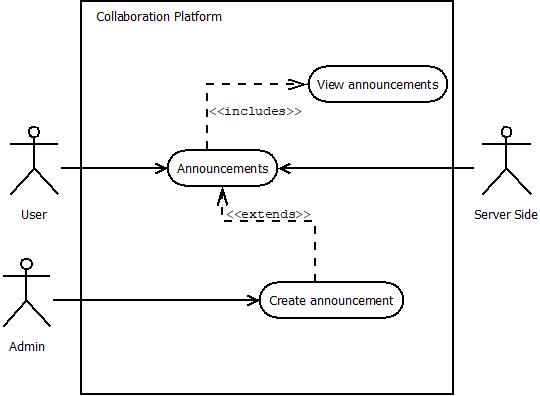
\includegraphics[scale=0.6]{figures/Announcements use case.jpeg}
    \caption{\textit{Use case} --- Announcements.}\label{fig:uc:announcements}
\end{figure}

\newpage

\section{Plataforma OutSystems}\label{sec:plataformaOutSystems}

A escolha da plataforma \textit{OutSystems~\cite{outsystems}}, para a implementação deste projeto baseia-se essencialmente no facto da mesma ser \textit{low-code},
apresentando vários benefícios essenciais para um projeto de curto prazo como o apresentado. A rapidez
com que é possível produzir peças de \textit{software}, as funcionalidades \textit{user-friendly} como \textit{drag and drop} e 
interfaces de utilizador pré-feitas e a possibilidade de produzir aplicações automaticamente através de
um simples clique, são elementos essenciais que levaram à escolha desta plataforma. 
\par
Cada \textit{endpoint} da aplicação está associado a um ecrã com o qual o utilizador interage, havendo uma navegabilidade entre ecrãs que permite que o utilizador visite os diferentes \textit{endpoints} da aplicação.
A criação e utilização de \textit{blocks} é uma das funcionalidades altamente vantajosas que a plataforma \textit{OutSystems~\cite{outsystems}} apresenta, 
visto que permite a reutilização deste componente ao longo da \textit{User Interface --- UI}.
\par
A construção da aplicação torna-se bastante rentável, em termos de tempo e facilidade do desenvolvimento, 
através da conjugação de conceitos como \textit{Widgets}, \textit{Screens} e \textit{Blocks} no domínio da  \textit{UI} 
e de conceitos como \textit{Server Actions} (ações executadas do lado do servidor), \textit{Client Actions} (ações executadas do lado do cliente) 
e \textit{Aggregates} (ação com o propósito de aceder à base de dados para retornar informações persistentes na mesma).
\par
Também é disponibilizado pela \textit{OutSystems~\cite{outsystems}}, um \textit{eSpace} por \textit{module} que contém elementos essenciais 
ao desenvolvimento, como os enunciados anteriormente.
\par
A base de dados está alojada numa \textit{cloud}, onde são guardadas todas as entidades dos vários módulos.
